% Created by tikzDevice version 0.10.1 on 2016-08-15 14:47:10
% !TEX encoding = UTF-8 Unicode
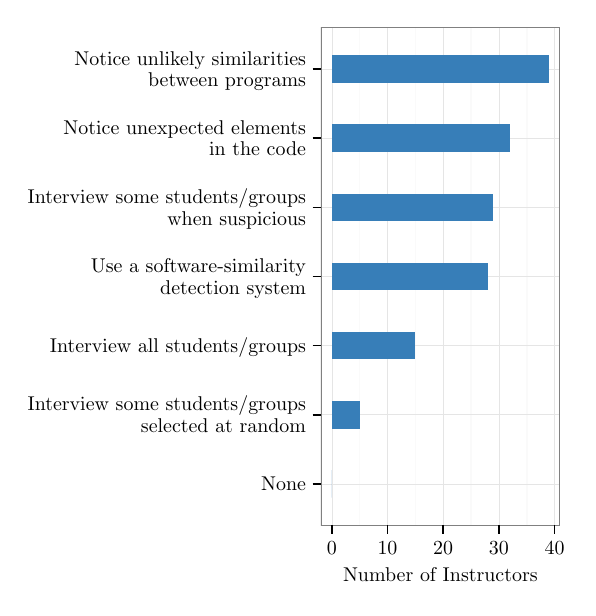
\begin{tikzpicture}[x=1pt,y=1pt]
\definecolor{fillColor}{RGB}{255,255,255}
\path[use as bounding box,fill=fillColor,fill opacity=0.00] (0,0) rectangle (195.13,202.36);
\begin{scope}
\path[clip] (  0.00,  0.00) rectangle (195.13,202.36);
\definecolor{drawColor}{RGB}{255,255,255}
\definecolor{fillColor}{RGB}{255,255,255}

\path[draw=drawColor,line width= 0.6pt,line join=round,line cap=round,fill=fillColor] (  0.00,  0.00) rectangle (195.13,202.36);
\end{scope}
\begin{scope}
\path[clip] (105.98, 22.52) rectangle (192.28,202.36);
\definecolor{fillColor}{RGB}{255,255,255}

\path[fill=fillColor] (105.98, 22.52) rectangle (192.28,202.36);
\definecolor{drawColor}{gray}{0.98}

\path[draw=drawColor,line width= 0.6pt,line join=round] (119.96, 22.52) --
	(119.96,202.36);

\path[draw=drawColor,line width= 0.6pt,line join=round] (140.08, 22.52) --
	(140.08,202.36);

\path[draw=drawColor,line width= 0.6pt,line join=round] (160.19, 22.52) --
	(160.19,202.36);

\path[draw=drawColor,line width= 0.6pt,line join=round] (180.31, 22.52) --
	(180.31,202.36);
\definecolor{drawColor}{gray}{0.90}

\path[draw=drawColor,line width= 0.2pt,line join=round] (105.98, 37.50) --
	(192.28, 37.50);

\path[draw=drawColor,line width= 0.2pt,line join=round] (105.98, 62.48) --
	(192.28, 62.48);

\path[draw=drawColor,line width= 0.2pt,line join=round] (105.98, 87.46) --
	(192.28, 87.46);

\path[draw=drawColor,line width= 0.2pt,line join=round] (105.98,112.44) --
	(192.28,112.44);

\path[draw=drawColor,line width= 0.2pt,line join=round] (105.98,137.41) --
	(192.28,137.41);

\path[draw=drawColor,line width= 0.2pt,line join=round] (105.98,162.39) --
	(192.28,162.39);

\path[draw=drawColor,line width= 0.2pt,line join=round] (105.98,187.37) --
	(192.28,187.37);

\path[draw=drawColor,line width= 0.2pt,line join=round] (109.90, 22.52) --
	(109.90,202.36);

\path[draw=drawColor,line width= 0.2pt,line join=round] (130.02, 22.52) --
	(130.02,202.36);

\path[draw=drawColor,line width= 0.2pt,line join=round] (150.14, 22.52) --
	(150.14,202.36);

\path[draw=drawColor,line width= 0.2pt,line join=round] (170.25, 22.52) --
	(170.25,202.36);

\path[draw=drawColor,line width= 0.2pt,line join=round] (190.37, 22.52) --
	(190.37,202.36);
\definecolor{fillColor}{RGB}{55,126,184}

\path[fill=fillColor] (109.90, 32.51) rectangle (109.90, 42.50);

\path[fill=fillColor] (109.90, 57.49) rectangle (119.96, 67.48);

\path[fill=fillColor] (109.90, 82.46) rectangle (140.08, 92.45);

\path[fill=fillColor] (109.90,107.44) rectangle (166.23,117.43);

\path[fill=fillColor] (109.90,132.42) rectangle (168.24,142.41);

\path[fill=fillColor] (109.90,157.40) rectangle (174.28,167.39);

\path[fill=fillColor] (109.90,182.37) rectangle (188.36,192.36);
\definecolor{drawColor}{gray}{0.50}

\path[draw=drawColor,line width= 0.6pt,line join=round,line cap=round] (105.98, 22.52) rectangle (192.28,202.36);
\end{scope}
\begin{scope}
\path[clip] (  0.00,  0.00) rectangle (195.13,202.36);
\definecolor{drawColor}{RGB}{0,0,0}

\node[text=drawColor,anchor=base east,inner sep=0pt, outer sep=0pt, scale=  0.72] at (100.58, 35.02) {None};

\node[text=drawColor,anchor=base east,inner sep=0pt, outer sep=0pt, scale=  0.72] at (100.58, 63.89) {Interview some students/groups};

\node[text=drawColor,anchor=base east,inner sep=0pt, outer sep=0pt, scale=  0.72] at (100.58, 56.11) {selected at random};

\node[text=drawColor,anchor=base east,inner sep=0pt, outer sep=0pt, scale=  0.72] at (100.58, 84.98) {Interview all students/groups};

\node[text=drawColor,anchor=base east,inner sep=0pt, outer sep=0pt, scale=  0.72] at (100.58,113.85) {Use a software-similarity};

\node[text=drawColor,anchor=base east,inner sep=0pt, outer sep=0pt, scale=  0.72] at (100.58,106.07) {detection system};

\node[text=drawColor,anchor=base east,inner sep=0pt, outer sep=0pt, scale=  0.72] at (100.58,138.82) {Interview some students/groups};

\node[text=drawColor,anchor=base east,inner sep=0pt, outer sep=0pt, scale=  0.72] at (100.58,131.05) {when suspicious};

\node[text=drawColor,anchor=base east,inner sep=0pt, outer sep=0pt, scale=  0.72] at (100.58,163.80) {Notice unexpected elements};

\node[text=drawColor,anchor=base east,inner sep=0pt, outer sep=0pt, scale=  0.72] at (100.58,156.02) {in the code};

\node[text=drawColor,anchor=base east,inner sep=0pt, outer sep=0pt, scale=  0.72] at (100.58,188.78) {Notice unlikely similarities};

\node[text=drawColor,anchor=base east,inner sep=0pt, outer sep=0pt, scale=  0.72] at (100.58,181.00) {between programs};
\end{scope}
\begin{scope}
\path[clip] (  0.00,  0.00) rectangle (195.13,202.36);
\definecolor{drawColor}{RGB}{0,0,0}

\path[draw=drawColor,line width= 0.6pt,line join=round] (102.98, 37.50) --
	(105.98, 37.50);

\path[draw=drawColor,line width= 0.6pt,line join=round] (102.98, 62.48) --
	(105.98, 62.48);

\path[draw=drawColor,line width= 0.6pt,line join=round] (102.98, 87.46) --
	(105.98, 87.46);

\path[draw=drawColor,line width= 0.6pt,line join=round] (102.98,112.44) --
	(105.98,112.44);

\path[draw=drawColor,line width= 0.6pt,line join=round] (102.98,137.41) --
	(105.98,137.41);

\path[draw=drawColor,line width= 0.6pt,line join=round] (102.98,162.39) --
	(105.98,162.39);

\path[draw=drawColor,line width= 0.6pt,line join=round] (102.98,187.37) --
	(105.98,187.37);
\end{scope}
\begin{scope}
\path[clip] (  0.00,  0.00) rectangle (195.13,202.36);
\definecolor{drawColor}{RGB}{0,0,0}

\path[draw=drawColor,line width= 0.6pt,line join=round] (109.90, 19.52) --
	(109.90, 22.52);

\path[draw=drawColor,line width= 0.6pt,line join=round] (130.02, 19.52) --
	(130.02, 22.52);

\path[draw=drawColor,line width= 0.6pt,line join=round] (150.14, 19.52) --
	(150.14, 22.52);

\path[draw=drawColor,line width= 0.6pt,line join=round] (170.25, 19.52) --
	(170.25, 22.52);

\path[draw=drawColor,line width= 0.6pt,line join=round] (190.37, 19.52) --
	(190.37, 22.52);
\end{scope}
\begin{scope}
\path[clip] (  0.00,  0.00) rectangle (195.13,202.36);
\definecolor{drawColor}{RGB}{0,0,0}

\node[text=drawColor,anchor=base,inner sep=0pt, outer sep=0pt, scale=  0.72] at (109.90, 12.16) {0};

\node[text=drawColor,anchor=base,inner sep=0pt, outer sep=0pt, scale=  0.72] at (130.02, 12.16) {10};

\node[text=drawColor,anchor=base,inner sep=0pt, outer sep=0pt, scale=  0.72] at (150.14, 12.16) {20};

\node[text=drawColor,anchor=base,inner sep=0pt, outer sep=0pt, scale=  0.72] at (170.25, 12.16) {30};

\node[text=drawColor,anchor=base,inner sep=0pt, outer sep=0pt, scale=  0.72] at (190.37, 12.16) {40};
\end{scope}
\begin{scope}
\path[clip] (  0.00,  0.00) rectangle (195.13,202.36);
\definecolor{drawColor}{RGB}{0,0,0}

\node[text=drawColor,anchor=base,inner sep=0pt, outer sep=0pt, scale=  0.72] at (149.13,  2.40) {Number of Instructors};
\end{scope}
\end{tikzpicture}
